The potential consequences of individual contamination scenarios can be quantified 
using the results from the contaminant transport simulations and a variety of impact 
assessment metrics. The \code{sim2Impact} subcommand performs impact assessments 
using the output threat ensemble database (ERD) from the \code{tevasim} subcommand. This analysis
provides all necessary network statistics for sensor network design (described 
in Chapter \ref{chap:sp}) as well as response actions, such as flushing hydrants and 
boosting disinfectant (described in Chapters \ref{chap:flush} and \ref{chap:booster}, respectively). 

A flowchart representation of the \code{sim2Impact} subcommand is shown in Figure \ref{fig:sim2Impact-flowchart}. 
The threat ensemble database (ERD) is the output from the \code{tevasim} subcommand and is 
required input for the \code{sim2Impact} subcommand. The consequences input parameters are supplied 
through the \code{sim2Impact} WST configuration file. Additional input data that describes 
the exposure and dose response models of a particular contaminant is required if a human health 
impact metric is used. These models are defined by parameters listed in a threat assessment input (TAI) file. 
More details on the TAI file are provided in the File Formats Section \ref{formats_taiFile}.  

\begin{figure}[h]
  \centering
  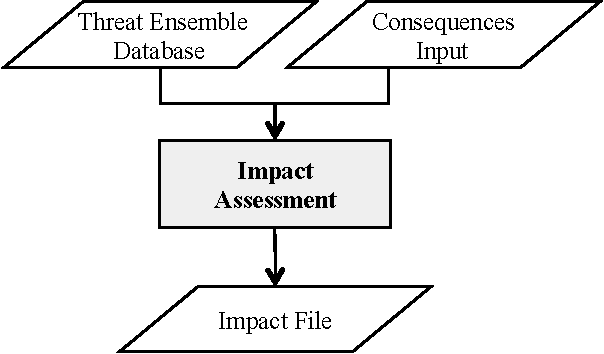
\includegraphics[scale=0.8]{graphics/sim2Impact_flowchart.pdf}
  \caption{Impact assessment flowchart.}
  \label{fig:sim2Impact-flowchart}
\end{figure}

Several impact metrics are included in the \code{sim2Impact} subcommand to reflect different 
criteria that decision makers could use in sensor network design or response actions. These metrics include:  
population dosed (PD), 
population exposed (PE),
population killed (PK), 
extent of contamination (EC),
%timed extent of contamination (TEC),
mass consumed (MC),  
volume consumed (VC), 
time to detection (TD) and
number of failed detections (NFD).
The equations used to compute the impact metrics are listed 
in Section \ref{impact_measures}.
Impact metrics are calculated at discrete time steps for a given 
contamination scenario. 
The discrete time steps are defined by the reporting time step and the duration of the water quality simulation.

Human health impacts (PD, PE and PK) can be estimated by combining 
the water quality simulations with exposure models. 
Contaminant-specific data are needed to accurately estimate the health endpoints. 
For many contaminants, reliable data are lacking, and the ensuing uncertainty 
in the results must be understood. More information on the human health impacts is 
provided in Section \ref{public_health_impacts}.

\section{Impact Metrics}\label{impact_measures}
Impact assessment results are calculated and stored in an impact file. 
This file is not typically read by a WST user, rather it is read by a sensor or 
response optimization routine. For each contamination scenario, the impact file 
contains a list of all the locations (nodes) in the network where a sensor might detect 
contamination from a specific scenario. Nodes that do not detect 
contamination are not included in the impact file for that specific scenario.
For each node that detects contamination, the impact file contains the detection time 
and consequence at that time, as measured by one of the impact metrics. 

The impact file is used as input for sensor placement optimization and during the 
optimization process of response actions, such as flushing hydrants and boosting disinfectant.   
When calculating impacts, a detection threshold can be specified such that contaminants 
are only detected above a specified concentration 
limit (the default limit is zero). Second, a response time can be specified in the \code{sim2Impact} configuration file, 
which accounts for the time needed to verify the presence of contamination 
(e.g., by field investigation), inform the public and/or initiate flushing, booster disinfection, 
or other response action (the default response time is zero). 
The contamination impact is computed at the time when the 
response has been initiated (the detection time plus response time), which is called 
the effective response time. Finally, a detection confidence can be defined, 
which specifies the number of sensors that must detect contamination from any given scenario 
before it is considered to be detected, at which time the impacts 
are calculated (the default is 1 sensor). 

The impact file contains four columns of information: 
\begin{itemize}
\item Column 1 contains the contamination scenario number, $a$
\item Column 2 contains the node location where contamination was detected, $i$
\item Column 3 contains the effective response time in minutes, $T'_i$
\item Column 4 contains the impact at the effective response time as measured by a specified metric, $d_{a,i}$
\end{itemize}
The impact file is documented in the File Formats Section \ref{formats_impactFile}.
The impact metric, $d_{a,i}$, is used directly in the sensor placement formulation (Equation \ref{eqn:eSP}),
the flushing formulation and the booster formulation.

The effective response time at node $i$, $T'_i$, is calculated using the following equation:
\begin{equation}
T'_i = \min{(t : \left|C_{n,t}>\textrm{detection limit}\right| \geq\textrm{detection confidence})}\Delta{T} + \textrm{response time}
\end{equation}
where $C_{n,t}$ is the contaminant concentration at node $n$ at time step $t$ for every node and time step in the water quality simulation.  
The concentration is typically expressed in units of milligrams per liter (mg/L). 
Concentration could also be a count of cells for a biological contaminant, where the units are cells/L or CFU/L (colony forming units/L).
The length of the reporting time step is denoted as $\Delta{T}$ and has units of time.
For detection, the concentration must be above the detection limit, and the number of detections must be above the detection confidence.
(Note $\left|C_{n,t}>\textrm{detection limit}\right|$ is the number of node, 
time step pairs where contaminant was detected above the detection limit, this includes detection at node $i$).

In the impact file, the impact at the end of the simulation time is included for each contamination scenario. 
Essentially, this is the impact if contamination was not detected at any node location, 
and is often referred to as the dummy sensor location.  The dummy sensor location is not a physical location in the network. For this entry, $i$ is set to -1, 
$T'_i$ is the time at the end of the water quality simulation and $d_{a,i}$ is 
the impact at the end of the simulation.

The impact, $d_{a,i}$, can be computed using one of the following metrics:
PD, PE, PK, EC, MC, VC, TD and NFD.
These metrics are defined in the following equations.  
In the equations, the effective response time step for node $i$, $t'_i$, equals $T'_i/\Delta{T}$, and
subscripts $n$, $t$ and $p$ are used to reference a specific node, time step and person, respectively.

\begin{itemize}

\item $\mathrm{PD}_{a,i}$, population dosed, is the total number of individuals that received a cumulative dose of contaminant 
above a specified threshold for scenario $a$ when contamination is detected at node $i$:

\begin{equation}
\mathrm{PD}_{a,i}=\sum_{n=1}^{N}\sum_{p=1}^{{\rm pop}_n}\delta_{n,p,t'_i}\textrm{ where } \delta_{n,p,t'_i} =
  \begin{cases}
   1 & \textrm{ if } d_{n,p,t'_i}> \textrm{ dose threshold } \\
   0 & \textrm{ otherwise }
  \end{cases}  
\end{equation} 
where $N$ is the number of nodes in the network,
$\mathrm{pop}_n$ is the population at node $n$ calculated using Equation \ref{eq:pop}, 
$d_{n,p,t'_i}$ is the cumulative dose for person $p$ at node $n$ at the effective response time step $t'_i$ calculated using Equation \ref{eq:dose} 
and dose threshold is defined by the user in the TAI file.

\item $\mathrm{PE}_{a,i}$, population exposed, is the number of individuals with a response 
to a contaminant for scenario $a$ when contamination is detected at node $i$:

\begin{equation}
\mathrm{PE}_{a,i}=\sum_{n=1}^{N}\mathrm{pop}_n\overline{r}_{n,t'_i} \equiv \sum_{n=1}^{N}(I_{n,t'_i}+D_{n,t'_i})
\end{equation}
where $N$ is the number of nodes in the network,
$\mathrm{pop}_n$ is the population at node $n$ calculated using Equation \ref{eq:pop} and 
$\overline{r}_{n,t'_i}$ is the percentage of the population at node $n$ at the effective 
response time step $t'_i$ that responds to a cumulative dose $d_{n,p,t'_i}$ calculated using Equation \ref{eq:rave}.
The variables, $I_{n,t'_i}$ and $D_{n,t'_i}$, represent the number of 
people in the infected and diseased states, respectively, at node $n$ 
at the effective response time step $t'_i$ computed from the disease progression model described in Section \ref{DPM}.

\item $\mathrm{PK}_{a,i}$, population killed, is the number of individuals killed by a contaminant 
for scenario $a$ when contamination is detected at node $i$:

\begin{equation}
\mathrm{PK}_{a,i}= \sum_{n=1}^{N}F_{n,t'_i}
\end{equation}
where $N$ is the number of nodes in the network and 
$F_{n,t'_i}$ represents the number of people in the fatality state (number of fatalities) 
at node $n$ at the effective response time step $t'_i$ 
computed from the disease progression model described in Section \ref{DPM}.

\item $\mathrm{EC}_{a,i}$, extent of contamination, is the length of contaminated pipe for scenario $a$ when contamination is detected at node $i$:

\begin{equation}
\mathrm{EC}_{a,i}=\sum_{n=1}^{N}L_{n,t'_i}\delta_{n,t'_i}\textrm{ where } \delta_{n,t'_i} =
  \begin{cases}
   1 & \textrm{ if } C_{n,t'_i}> \textrm{ detection limit } \\
   0 & \textrm{ otherwise }
  \end{cases}  
\end{equation}
where $N$ is the number of nodes in the network,
$L_{n,t'_i}$ is the length of all pipes connected to node $n$ with flow starting at node $n$ at the effective response time step $t'_i$
and $C_{n,t'_i}$ is the contaminant concentration at node $n$ at the effective response time step $t'_i$.
An entire pipe is considered contaminated if the contaminant enters the pipe. 

%\item $T\mathrm{EC}_{a,i}$, timed extent of contamination, is the length of contaminated pipe for scenario $a$ when contamination is detected at node $i$ and 
%includes the length of contaminated pipe each time a node is contaminated, up to the time when contamination is detected:
 
%\begin{equation}
%T\mathrm{EC}_{a,i}=\sum_{n=1}^{N}\sum_{t=1}^{t'_i}L_{n,t}\delta_{n,t}\text{ where } \delta_{n,t} =
%  \begin{cases}
%   1 & \text{ if } C_{n,t}> \text{ detection limit } \\
%   0 & \text{ otherwise }
%  \end{cases}  
%\end{equation}
%where $N$ is the number of nodes in the network,
%$L_{n,t}$ is the length of all pipes connected to node $n$ with flow starting at node $n$ at time step $t$ 
%and $C_{n,t}$ is the contaminant concentration at node $n$ at time step $t$. 
%An entire pipe is considered contaminated if the contaminant enters the pipe. This metric is only intended to be used 
%within the flushing response optimization routine, which only uses the the impact at the end of the simulation time. 

\item $\mathrm{MC}_{a,i}$, mass consumed, is the cumulative mass of the contaminant consumed 
via the nodal demands for scenario $a$ when contamination is detected at node $i$:

\begin{equation}
\mathrm{MC}_{a,i}=\sum_{n=1}^{N}\sum_{t=1}^{t'_i}C_{n,t}q_{n,t}\Delta{T}
\end{equation}
where $N$ is the number of nodes in the network,
$C_{n,t}$ is the contaminant concentration at node $n$ at time step $t$, 
$q_{n,t}$ is the demand at node $n$ at time step $t$ and 
$\Delta{T}$ is the length of the reporting time step. In other words, this metric 
measures the mass of the contaminant removed from the system at node $i$ via nodal 
demand between the start of the simulation and time ${t'_i}$.

\item $\mathrm{VC}_{a,i}$, volume consumed, is the cumulative volume of contaminated water consumed 
via nodal demand for scenario $a$ when contamination is detected at node $i$:

\begin{equation}
\mathrm{VC}_{a,i}=\sum_{n=1}^{N}\sum_{t=1}^{t'_i}q_{n,t}\Delta{T}\delta_{n,t}\textrm{ where } \delta_{n,t} =
  \begin{cases}
   1 & \textrm{ if } C_{n,t}> \textrm{ detection limit } \\
   0 & \textrm{ otherwise }
  \end{cases}  
\end{equation}
where $N$ is the number of nodes in the network,
$C_{n,t}$ is the contaminant concentration at node $n$ at time step $t$, 
$q_{n,t}$ is the demand at node $n$ at time step $t$ and 
$\Delta{T}$ is the length of the reporting time step. In other words, this metric 
measures the volume of the contaminant removed from the system at node $i$ via 
nodal demand between the start of the simulation and time ${t'_i}$.

\item $\mathrm{TD}_{a,i}$, time to detection, is the time from the beginning of scenario $a$ until contamination is first detected at a node $i$.

\begin{equation}
\mathrm{TD}_{a,i}=T'_i-\textrm{ injection start time}
\end{equation}
where $T'_i$ is the effective response time.

\item $\mathrm{NFD}_{a,i}$, number of failed detections, is a binary value to indicate 
the detection of scenario $a$ at node $i$:  

\begin{equation}
\mathrm{NFD}_{a,i}=
  \begin{cases}
   1 & \textrm{ if scenario } a \textrm{ is not detected at node }i \\
   0 & \textrm{ otherwise }
  \end{cases}  
\end{equation}
where the total impact is given a value of 1 if scenario $a$ is not detected at node $i$ 
or the value of 0 if scenario $a$ is detected at node $i$. 
Since the impact file only lists nodes which detect scenarios, all node, time pairs 
have a total impact of 0, except for the dummy location (i = -1), which is given a value of 1.

\end{itemize}

\section{Human Health Impact Model}\label{public_health_impacts}

The human health impact model is used to compute PD, PE and PK.
In order to calculate these metrics, an estimate of the population 
ingesting water and the cumulative dose and response for each individual at each node 
is required. A disease progression model is used to compute the population 
susceptible, infected, diseased and killed given a cumulative dose of contaminant. 
Input parameters for the human health impact model are stored in a TAI file.
The TAI file format is described in Section \ref{formats_taiFile}. 
Additional information on human health impact models can be 
found in the EPA compendium report \citep{TEVASPOTCompendium10}.

\subsection{Population}
\if 0
The population at each network node can either be defined explicitly or calculated based on the 
average amount of water consumed at the node. 
The demand-based calculation uses the demand patterns specified for each node.
The average water consumed at node $n$, $\overline{q}_n$, is computed by:
\begin{equation}
\overline{q}_n=\dfrac{\sum_{k=1}^{K}\sum_{t=1}^{lcm_n}qbase_n m_n(k,t\bmod L(k))}{lcm_n}\label{eq:qave}
\end{equation}
where $K$ is the number of demand patterns at node $n$, 
$L(k)$ is the number of time steps in pattern $k$,
$lcm_n$ is the least common multiple of the demand patterns time steps for node $n$, 
$qbase_n$ is the base demand at node $n$ and 
$m_n(k,t\bmod L(k))$ is the demand multiplier specified in pattern $k$ for node $n$ at time $t\bmod L(k)$. 
For example, if a node has two demand patterns specified in the EPANET input (INP) file, and 
one pattern repeats every 6 hours and the other repeats every 12 hours, the first 
pattern will be repeated once, making its total duration effectively 12 hours. 
If any $m_n(k,t\bmod L(k))$ value is less than 0, then that node's population is 0.  
\fi

The population at each network node can either be defined explicitly in the TAI 
file using a population file or calculated based on the demand at each node.  
The population file has one line per node. Each line contains the node ID followed by the population value for that node.
For the demand-based calculation, it is assumed that all water leaving the network is consumed by the population.
The water consumption is more than just the ingestion of water by people, since it includes all uses of water, such 
as domestic, commercial, industrial, agricultural and others. 
Therefore, the population at node $n$, $\mathrm{pop}_n$, is computed using the following equation:
\begin{equation}
\mathrm{pop}_n=\dfrac{\overline{q}_n}{R}\label{eq:pop}
\end{equation}
where $\overline{q}_n$ is the average volume of water consumed at node $n$ per day and $R$ 
is the average volume of water consumed per capita per day. The variable, $R$, is set in the TAI file.
A USGS report provides usage rates by state and gives a nationwide 
average of 179 gallons per capita per day \citep{USGS04}. Often 200 
gallons per capita per day is used for $R$. The population is 
assumed to be constant over time.  

\subsection{Cumulative Dose}

At each node, the total number of people potentially ingesting water is given 
by $\mathrm{pop}_n$. In order to compute the cumulative dose, additional information 
is needed, including when and how much a person drinks. Ingestion 
timing and volume models are used to make this calculation. 
Additional information on the ingestion and volume models can be found in \citet{DavJan08}.
Three different ingestion timing models are available: 
\begin{itemize}
\item Demand-based (D24): assumes that tap water is ingested at every time step in an 
amount proportional to the total water demand at that node. 
\item Fixed (F5): assumes that tap water is ingested at five fixed times during a 
day. These times are set to the typical starting times for the three major meals on weekdays (7:00, 
12:00 and 18:00) and times halfway between these meals (9:30 and 15:00).  
\item Probabilistic (P5): also assumes that tap water is ingested at five times per day 
at major meals and halfway between them, but it uses a probabilistic approach 
to determine meal times. This is based on data from the American Time-Use Survey 
(ATUS) \citep{ATUS}. 
\end{itemize}
In addition, there are two ingestion volume models: 
\begin{itemize}
\item Mean (M): assumes the same average quantity of tap water is ingested by all individuals in the population who consume tap water.  
\item Probabilistic (P): uses a probabilistic approach to estimate the volume ingested by individual people.
\end{itemize}
The ingestion timing model and the volume model are set in the TAI file.
The D24 ingestion timing model is used only with the M volume model. 
Either the M or P volume models can be used with the F5 and P5 timing models. 
The volume models are used to determine a per capita ingestion volume, $\hat{V}_{n,p}$, 
in liters/day for each person $p$ at node $n$. 
When using the M volume model, $\hat{V}_{n,p}$ is the same for each person and is commonly set to 1 to 2 liters/day. 
When using the P volume model, $\hat{V}_{n,p}$ can be different for each person. 
In each case, the volume ingested per day, $\hat{V}_{n,p}$, must be converted to 
a volume ingested per time step, $V_{n,p,t}$, to calculate cumulative dose for each time step.

When using the D24 ingestion timing model, $V_{n,p,t}$ is related to the demand at that node. 
The fraction of demand water, $rho_{n,t}$, that is ingested at node $n$ at time step $t$, 
considering the entire length of the simulation, is computed by:
\begin{equation}
\rho_{n,t}=\dfrac{q_{n,t}}{\sum_{t=1}^{\mathrm{nsteps}}q_{n,t}}\mathrm{nsteps}\Delta{T}
\end{equation}
where $q_{n,t}$ is the demand at node $n$ at time step $t$, $\mathrm{nsteps}$ is number 
of time steps in the entire simulation and $\Delta{T}$ is the length of the reporting time step. 
The length of the simulation equals $\mathrm{nsteps}\Delta{T}$.
The volume $V_{n,p,t}$ is then computed using:
\begin{equation}
V_{n,p,t}=\rho_{n,t}\hat{V}_{n,p}\label{eq:VD24}
\end{equation}

When using the F5 and P5 ingestion timing models, $\hat{V}_{n,p}$ is divided equally among each time step in which water is ingested.
\begin{equation}
V_{n,p,t}=
  \begin{cases}
   \hat{V}_{n,p}/5 & \textrm{if } t \in \textrm{\{ingestion time steps\} } \\
   0 & \textrm{otherwise}
  \end{cases}
  \label{eq:VF5P5}
\end{equation} 
The set of ingestion time steps is calculated by dividing the ingestion times by 
the length of the reporting time step. This value is rounded down to the nearest discrete time step. 
The simulation start time should first be subtracted from the ingestion times.  
For example, if the set of ingestion times are defined using the F5 model as \{7:00, 9:30, 
12:00, 15:00 and 18:00\}, the start time is 4:15 and the reporting time step is 
a half hour, the set of ingestion time steps are \{5, 10, 15, 21 and 27\}.

The cumulative dose for person $p$ at node $n$ at time step $t$, $d_{n,p,t}$, is computed using the following equation:
\begin{equation}
d_{n,p,t}=\sum_{j=1}^{t}C_{n,j}V_{n,p,j}\label{eq:dose}
\end{equation}
where $V_{n,p,j}$ is calculated using Equation \ref{eq:VD24} or Equation \ref{eq:VF5P5} and 
$C_{n,j}$ is the contaminant concentration in the water at node $n$ at 
time step $j$ as predicted by the water quality simulations. Cumulative dose is given in number 
of organisms or mass in milligrams.

\subsection{Response}
Dose-response functions are used to predict the percentage of the population that might 
experience a particular health outcome after receiving a specific cumulative dose. 
Two dose-response functions, $r(d_{n,p,t})$, are available in the \code{sim2Impact} subcommand:
\begin{itemize}
\item Log-Probit model:
\begin{equation}
r(d_{n,p,t})=\Phi (\beta \ln(d_{n,p,t} \mathrm{LD50}))\label{eq:probit}
\end{equation}
where $\Phi$ is the cumulative distribution function of a standard normal random variable, 
$\beta$ is related to the slope of the curve, 
$\mathrm{LD50}$ (or $\mathrm{ID50}$ for biological agents) is the dose at which 50\% of the exposed population would die 
and $d_{n,p,t}$ is calculated using Equation \ref{eq:dose}. The parameters $\beta$ and $\mathrm{LD50}$ are set in the TAI file.
\item Generic logistic function:
\begin{equation}
r(d_{n,p,t})=\dfrac{a(1+me^{-d_{n,p,t}/\tau})}{1+\eta e^{-d_{n,p,t}/\tau}} \textrm{~where~} \eta=e^{\mathrm{LD50}/\tau}-2 \label{eq:general}
\end{equation}
where $a$, $m$, $\eta$ and $\tau$ are function coefficients used to fit the model to available data 
and $d_{n,p,t}$ is calculated using Equation \ref{eq:dose}. 
The parameters $a$, $m$, $\eta$ and $\tau$ are set in the TAI file.
\end{itemize}

The average response, $\overline{r}_{n,t}$, of the population at node $n$ at time step $t$ is calculated by:
\begin{equation}
\overline{r}_{n,t}=\dfrac{\sum_{p=1}^{\textrm{pop}_n}r(d_{n,p,t})}{\textrm{pop}_n}\label{eq:rave}
\end{equation}
where $\textrm{pop}_n$ is calculated using Equation \ref{eq:pop} and $r(d_{n,p,t})$ is calculated 
using Equation \ref{eq:probit} or Equation \ref{eq:general}.

\subsection{Disease Progression Model}\label{DPM}
To track how the population at each node responds to a specified contaminant over time, a disease 
progression model is used. Given the percentage of people at each node who would become 
ill after being exposed to the contaminant, disease transmission models predict 
how the disease would progress over time. Disease models are used to predict the 
number of people at each node susceptible to illness from the contaminant ($S$), 
exposed to a lethal or infectious dose ($I$), experiencing symptoms of disease ($D$) 
and either recovering ($R$) or being fatally impacted ($F$). These equations assume that the recovered 
population does not rejoin the susceptible population.
These quantities are predicted at each node over time according to the following 
differential equations:
\begin{align}
\dfrac{dS}{dt} &= - \lambda S\label{eq:S}\\
\dfrac{dI}{dt} &= \lambda S - \sigma I\\
\dfrac{dD}{dt} &= \sigma I - (\alpha+\nu)D\\
\dfrac{dR}{dt} &= \nu D\\
\dfrac{dF}{dt} &= \alpha{D}
\end{align}
where 
$\lambda$ is the per capita rate of infection,
$\sigma$ is the per capita rate at which infected move to diseased,
$\alpha$ is the per capita disease induced untreated death rate and
$\nu$ is the per capita recovery rate, or the rate at 
which diseased moved to recovered or fatal states.  

The infection rate, $\lambda$, is given by:
\begin{equation}
\lambda_{n,t}=\dfrac{dr_{n,p,t}}{dt}\dfrac{S_{n,0}}{S_{n,t}}
\end{equation}
where $r(d_{n,p,t})$ is calculated using Equation \ref{eq:probit} or Equation \ref{eq:general} and 
$S$ is calculated by Equation \ref{eq:S}.

In the TAI file, the LATENCY TIME is the inverse of $\sigma$, 
the FATALITY RATE is $\alpha$ and the FATALITY TIME is the inverse of $\nu$. 
For more detail on the disease progression model and health impacts, see \citet{MurUbeJan06}.

\if 0
The population at each node starts out as susceptible $S$. The number of people 
at each node is calculated using Equation \ref{eq:pop}. 
As the population at each node has a response to a contaminant, individuals are moved to the infected 
state $I$. The average response is calculated using Equation \ref{eq:rave}. 
After a specified latency time, the infected population
is moved to the diseased state $D$. After a specified fatality time, a fraction 
of the diseased population is moved to the fatality state $F$. 
The population in each state is calculated using the following equations. 

\begin{align}
S_n(t) &= S_n(t-1)-sout_n(t)\\
I_n(t) &= I_n(t-1)+sout_n(t)-iout_n(t)\\
D_n(t) &= D_n(t-1)+iout_n(t)-dout_n(t)\\
R_n(t) &= dout_n(t)�(1-R_f)\\
F_n(t) &= dout_n(t)�R_f\label{eq:DPM}
\end{align}

where $R_f$ is the fraction of the diseased population that dies,
$sout$ is the percentage of the population at node $n$ that needs to move from $S$ to $I$ at time step $t$, 
$iout$ is the percentage of the population at node $n$ that needs to move from $I$ to $D$ at time step $t$, and 
$dout$ is the percentage of the population at node $n$ that needs to move from $D$ to $F$ at time step $t$.

The quantities $sout$, $iout$ and $dout$ are calculated using the following equation:
\begin{align}
sout_n(t) &=
  \begin{cases}
   \overline{r}_n(t)-\overline{r}_n(t-1) \text{ if } t>1 \\
   1 \text{ otherwise }
  \end{cases}\\
iout_n(t) &=
  \begin{cases}
   \overline{r}_n(t-t_L)-\overline{r}_n(t-t_L-1) \text{ if } t>t_L+1 \\
   0 \text{ otherwise }
  \end{cases}\\
dout_n(t) &=
  \begin{cases}
   \overline{r}_n(t-t_L-t_F)-\overline{r}_n(t-t_L-t_F-1) \text{ if } t>t_L+t_F+1 \\
   0 \text{ otherwise }
  \end{cases}
\end{align}

where $\overline{r}_n(t)$ is the average response calculated using Equation \ref{eq:rave},
$t_L$ is the latency time step and 
$t_F$ is the fatality time step.
The latency time steps is calculated by dividing the latency time by the length of the reporting time step. This value is rounded down to the nearest discrete time step. 
The fatality time step is calculated in a similar manner.
\fi

\section{\code{sim2Impact} Subcommand}

The \code{sim2Impact} subcommand is executed using the following command line:
\begin{unknownListing}
wst sim2Impact <configfile> 
\end{unknownListing}
where \code{configfile} is a WST configuration file in the YAML format. 

The \code{---help} option prints information about this subcommand, such as usage,
arguments and a brief description:

\begin{unknownListing}
wst sim2Impact --help
\end{unknownListing}

\subsection{Configuration File}

The \code{sim2Impact} subcommand generates a template configuration file using the following command line:
\begin{unknownListing}
wst sim2Impact --template <configfile>
\end{unknownListing}

The \code{sim2Impact} WST configuration template is shown in Figure \ref{fig:sim2Impact_template}. 
Brief descriptions of the options are included in the configuration template after the \# sign. 

\begin{figure}[h!]
  \unknownInputListing{examples/sim2Impact_config.yml}{}{1}{13}
  \caption{The \code{sim2Impact} configuration template file.}
  \label{fig:sim2Impact_template}
\end{figure}

\subsection{Configuration Options}

Full descriptions of the WST configuration options used by the \code{sim2Impact} subcommand are listed below.
\begin{description}[topsep=0pt,parsep=0.5em,itemsep=-0.4em]
  \item[{impact}]\hfill
  \begin{description}[topsep=0pt,parsep=0.5em,itemsep=-0.4em]
    \item[{erd file}]\hfill
\\The name of the ERD database file that contains the 
                contaminant transport simulation results. It is 
                created by running the \code{tevasim} subcommand.
                Multiple ERD files (entered as a list, i.e., [<file1>, <file2>]) can be combined to
                generate a single impact file. This can be used to combine
                simulation results from different types of contaminants, in
                which the ERD files were generated from different
                TSG files.
                
                Required input.
    \item[{metric}]\hfill
\\The impact metric used to compute the impact file. Options
                include EC, MC, NFD, PD, PE, PK, TD or VC. One impact file 
                is created for each metric selected. These metrics are 
                defined in Section \ref{impact_measures}.
                
                Required input.
    \item[{tai file}]\hfill
\\The name of the TAI file that contains health impact information. 
                The TAI file format is documented in File Formats Section \ref{formats_taiFile}.
                
                Required input if a public health metric is used (PD, PE or PK).
    \item[{response time}]\hfill
\\The number of minutes that are needed to respond to the
                detection of a contaminant. This represents the time that it takes
                a water utility to stop the spread of the contaminant in the network and 
                eliminate the consumption of contaminated water. As the response time increases,
                the impact increases because the contaminant affects the network
                for a greater length of time.  
                
                Required input, default = 0 minutes.
    \item[{detection limit}]\hfill
\\The minimum concentration that must be exceeded before a sensor can detect a contaminant.
                There must be one threshold for each ERD file. The units of
                these detection limits depend on the units of the contaminant
                simulated for each ERD file (e.g., number of cells of a
                biological agent).  
                
                Required input, default = 0.
    \item[{detection confidence}]\hfill
\\The number of sensors that must detect an incident before
                the impacts are calculated.  
                
                Required input, default = 1 sensor.
  \end{description}
  \item[{configure}]\hfill
  \begin{description}[topsep=0pt,parsep=0.5em,itemsep=-0.4em]
    \item[{output prefix}]\hfill
\\The prefix used for all output files.
                
                Required input.
    \item[{output directory}]\hfill
      \\The output directory to store the results.
    \item[{debug}]\hfill
\\The debugging level (0 or 1) that indicates the amount of debugging 
                information printed to the screen, log file and output yml file. 
                
                Optional input, default = 0 (lowest level).
  \end{description}
\end{description}


\subsection{Subcommand Output}

The \code{sim2Impact} subcommand creates 
two output files, one is in the YAML file format and the other is a log file.
The YAML file is called <output prefix>sim2Impact\_output.yml 
and the log file is <output prefix>sim2Impact\_output.log.  
The YAML file contains the names of the impact file(s), the 
ID file(s), the nodemap file and the scenario map file, 
as well as the run date and the CPU time.
These files are described below.
The log file contains basic debugging information.

\begin{itemize}
\item Impact file: One impact file is generated for each of the impact metrics 
specified. The file contains the observed impact at each location where a 
contamination scenario could be observed by a potential sensor. This file is not 
intended to be read by users, but it is used later for sensor placement or other 
response optimization. The impact file is documented in the File Formats Section \ref{formats_impactFile}.
\item ID file: For each impact file (e.g., wst\_Net3\_mc.impact ), a corresponding ID 
file is generated to map the location IDs back to the network node labels. This file is not 
intended to be read by users, since it is used internally by the software code. 
\item Nodemap file: The nodemap file maps sensor placement IDs to the 
network node labels (defined by EPANET). This file is not 
intended to be read by users, since it is used internally by the software code. 
The nodemap file is documented in the File Formats Section \ref{formats_nodeFile}.
\item Scenario map file: The scenario map file maps contamination scenario IDs to the 
network node labels (defined by EPANET). This file is not 
intended to be read by users, since it is used internally by the software code. 
The scenario map file is documented in the File Formats Section \ref{formats_scenarioFile}.
\end{itemize}

\section{Impact Assessment Examples}\label{sim2impact_example}

After simulating the fate and transport of contaminants in a water distribution network, 
the output can be used to quantify the impacts of the contamination incidents. 
An ERD file and a configuration file are required to run the \code{sim2Impact} subcommand. 
In the following examples, the EPANET Example Network 3 is used. The output database, Net3.erd, 
from the first \code{tevasim} subcommand example is used to compute the impact assessments.

\subsection{Example 1}

Figure \ref{fig:sim2Impact_ex1} shows the configuration file, sim2Impact\_ex1.yml, 
for the first \code{sim2Impact} subcommand example. This example computes an impact assessment, based on Net3.erd, 
for the mass consumed (MC), volume consumed (VC), extent of contamination (EC), time to detection (TD), 
number of failed detections (NFD) and population exposed (PE) impact metrics. The TAI file, Net3\_bio.tai, 
is added to define the human health impact for a biological contaminant. The response time, detection
limit and detection confidence are all set at the default values (i.e., 0, 0, 1, respectively).

\begin{figure}[h!]
  \unknownInputListing{../../examples/sim2Impact_ex1.yml}{}{1}{11}
  \caption{The \code{sim2Impact} configuration file for example 1.}
  \label{fig:sim2Impact_ex1}
\end{figure}

The example can be executed using the following command line:

\begin{unknownListing}
wst sim2Impact sim2Impact_ex1.yml
\end{unknownListing}

For each impact metric, an impact file (e.g., Net3\_pe.impact) and a corresponding 
ID file is generated (e.g., Net3\_pe.impact.id). For each contamination scenario (shown in column 1 
after a two line header), the impact file contains a list of nodes in the 
network (column 2) where a sensor might detect that contamination. For each 
such node, the impact file contains the detection time (column 3) and the 
total impact (column 4) given a sensor at that node is the first to detect 
contamination from that scenario.  

\FloatBarrier 
\subsection{Example 2}

The second example using the \code{sim2Impact} subcommand investigates the 
effect of changing the response time and detection limit on a specific impact metric, MC. 
The example 2 configuration file, sim2Impact\_ex2.yml, is shown in Figure \ref{fig:sim2Impact_ex2}. 
This example uses a 60-minute response time and a detection limit of 0.1. 
Note that the units for detection limit are the same as for the 
mass values specified in the TSG file. 

\begin{figure}[h!]
  \unknownInputListing{../../examples/sim2Impact_ex2.yml}{}{1}{11}
  \caption{The \code{sim2Impact} configuration file for example 2.}
  \label{fig:sim2Impact_ex2}
\end{figure}

The example can be executed using the following command line:
\begin{unknownListing}
wst sim2Impact sim2Impact_ex2.yml
\end{unknownListing}

\FloatBarrier 
\if 0
\subsection{Example 3}

The third \code{sim2Impact} example calculates the MC impact metric from multiple ERD files. 
The ERD files, Net3.erd and Net3\_EColi\_TSB.erd, are from the two \code{tevasim} subcommand examples. 
The \code{sim2Impact} example 3 configuration file, sim2Impact\_ex3.yml, is shown in Figure \ref{fig:sim2Impact_ex3}. 
The response time and detection confidence options are set to the default values. 
The detection threshold for the contaminant described in Net3.erd is 3000000 and 0.1 for 
the contaminant described in Net3\_Ecoli\_TSB.erd. \citet{MurrayBerryHart2006} use this technique to
combine data from different types of contamination scenarios into a single impact metric.

\begin{figure}[h!]
  \unknownInputListing{../../examples/sim2Impact_ex3.yml}{}{1}{11}
  \caption{The \code{sim2Impact} configuration file for example 3.}
  \label{fig:sim2Impact_ex3}
\end{figure}

The example can be executed using the following command line:
\begin{unknownListing}
wst sim2Impact sim2Impact_ex3.yml
\end{unknownListing}


\FloatBarrier 
\fi
\subsection{Example 3}

The \code{sim2Impact} example 3 calculates the impact associated with multi-species
contamination incidents. The msx species option specifies which species concentration profile 
to use to calculate impact metrics. This option is required for multi-species contamination scenarios 
created by the \code{tevasim} subcommand. The configuration file for the multi-species example, 
sim2Impact\_ex3.yml, is shown in Figure \ref{fig:sim2Impact_ex3}. This example uses an ERD 
file created by EPANET-MSX and computes the MC impact metric for the $E.~coli$ species. The
response time, detection limit and detection confidence are all set at their default values.

\begin{figure}[h!]
  \unknownInputListing{../../examples/sim2Impact_ex3.yml}{}{1}{11}
  \caption{The \code{sim2Impact} configuration file for example 3.}
  \label{fig:sim2Impact_ex3}
\end{figure}

The example can be executed using the following command line:
\begin{unknownListing}
wst sim2Impact sim2Impact_ex3.yml
\end{unknownListing}

